\chapter{L'arborescence}

L'arborescence sous Linux correspond à la manière sont agencés les dossiers (directory en anglais) les uns par rapport aux autres.

\begin{center}
	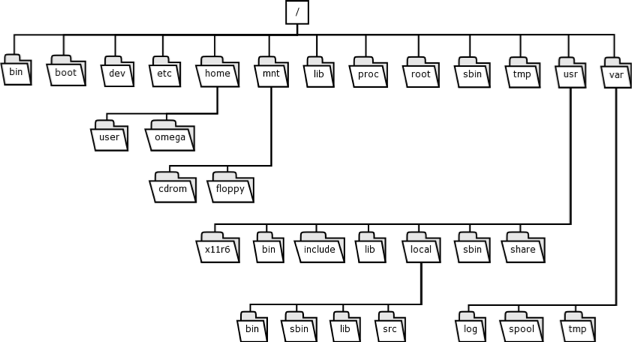
\includegraphics[width=0.7\textwidth]{Images/arborescence.png}
	\captionof{figure}{Arborescence d'un système GNU/Linux}
\end{center}

Vous l'aurez peut être remarqué mais tous les dossiers mènent à /. Ce dossier a pour petit nom, root. Il est ce que l'on appelle la racine du système. De ce dossier découle une floppé d'autre. Chacun à son utilité, nous allons voir les "plus important"
\begin{itemize}
	\item home : ce dossier contient les fichiers des utilisateurs. C'est ici que se situe les données des utilisateurs.
	\item 
\end{itemize}
